%!TEX root = ../thesis.tex
% ******************************* Thesis Appendix B ********************************

\chapter{Chip and Pixel Bias Voltage}
\label{appendix:bias}

There are two ways to apply bias voltage to the sensors: either by the chip guard ring or the pixel guard ring, as shown in Fig. \ref{img:GuardRing}.

\begin{figure}[h!] 
\centering
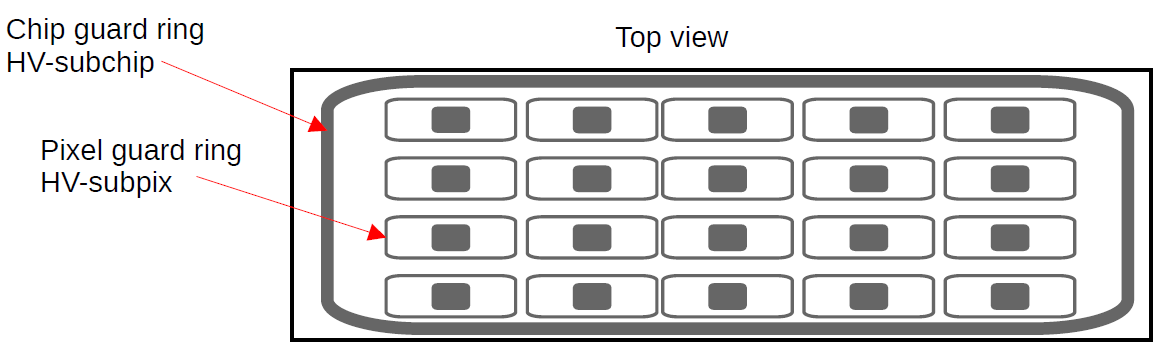
\includegraphics[width=0.75\linewidth]{Appendix2/GuardRing.png}
\caption{An simplified front view of the TelePix2 sensor\cite{testupdate}. Chip guard ring and pixel guard rings, from which the bias voltage can be applied.}
\label{img:GuardRing}
\end{figure}

%When bias voltage was applied through the pixel guard ring, the voltage on the chip guard ring was measured, and vice versa. The result is shown in the figure below.

\begin{figure}[h!]
\centering
\begin{subfigure}{.49\textwidth}
  \centering
  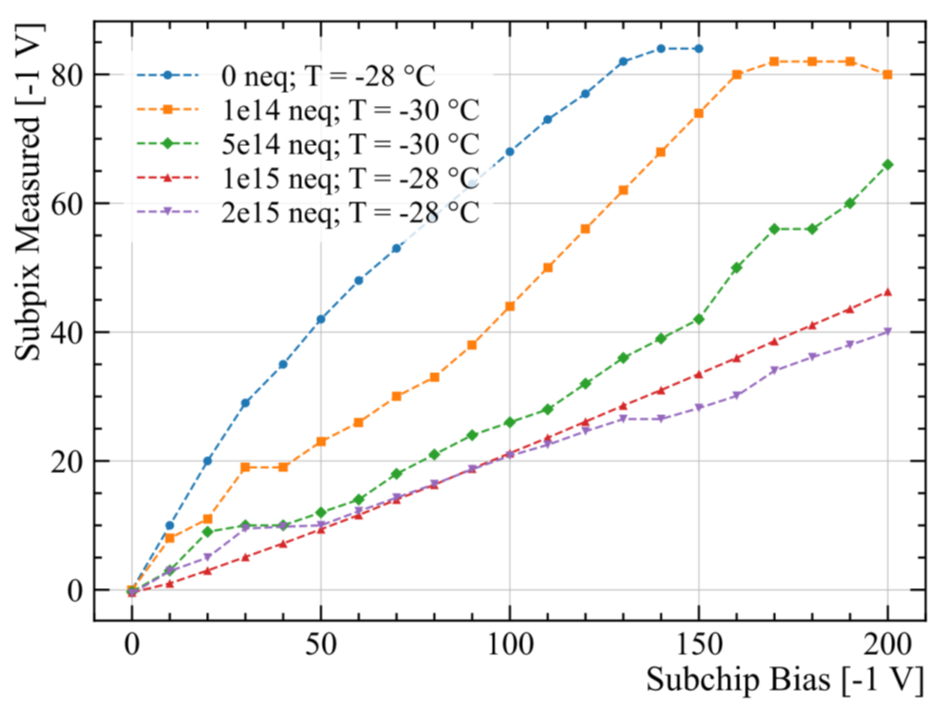
\includegraphics[width=1.0\linewidth]{Appendix2/ChipToPix.png}
  \caption{Voltage applied on chip and measured on pixel.}
  %\label{fig:sub1}
\end{subfigure}
\begin{subfigure}{.49\textwidth}
  \centering
  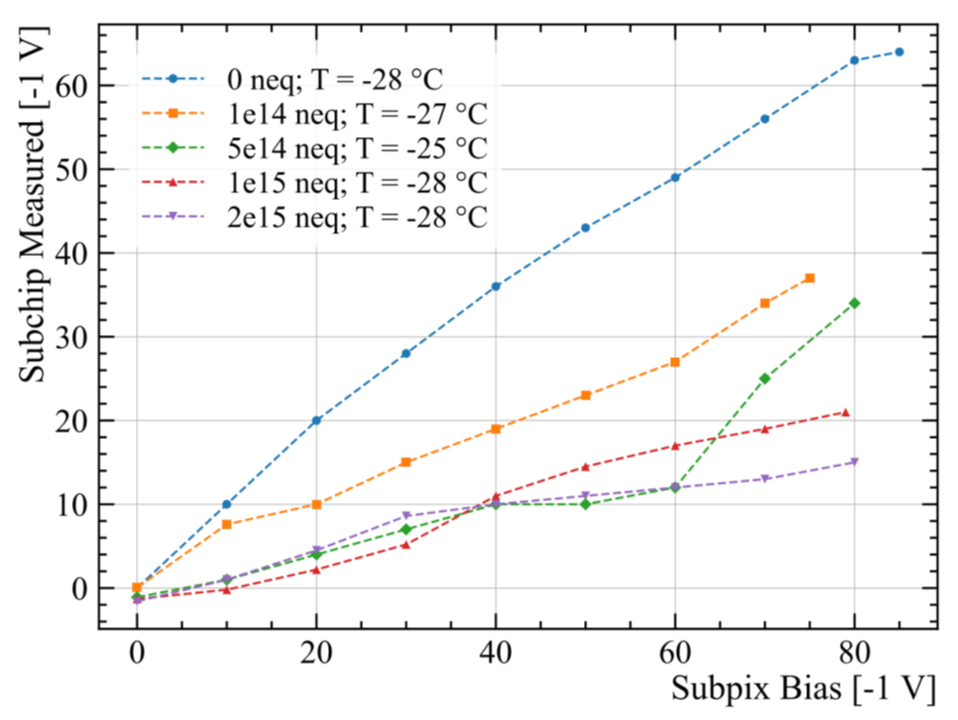
\includegraphics[width=1.0\linewidth]{Appendix2/PixToChip.png}
  \caption{Voltage applied on pixel and measured on chip.}
  %\label{fig:sub2}
\end{subfigure}
\caption{The measured voltage on pixel guard ring when bias was applied on chip guard ring, and vice versa\cite{testupdate}. Note that the values are not one-to-one corresponded.}
\label{img:PixChipConvert}
\end{figure}